\chapter{Game Analysis}
\label{GameAnalysis}

In Chapter \ref{GameDescription}, we explored the rules and gameplay mechanics of Quoridor.
As we progress, this chapter aims to deepen our understanding by analyzing Quoridor from a
theoretical and computational perspective.

In this chapter, we will classify Quoridor within the realm of strategic games, examine its game tree,
state-space and tree complexity, and explore the implications of these factors on gameplay and
artificial intelligence application.

\section{Classification of Quoridor}

Quoridor can be characterized as a discrete, deterministic, zero-sum, sequential, game with perfect
information \citep{Glendenning2002MasteringQ}, and therefore, a combinatorial game \citep{GameTheoryBook}. 

\subsection{Discrete}
In every turn of the game, each player has a finite number of moves and wall placements. These are limited by the game state (already placed walls and moved pawns) and the rules of the game. The game-tree of Quoridor has finite number of nodes (e.g Figure \ref{fig:GameTree}).

\subsection{Deterministic}
Quoridor has no random elements or chance involved in the gameplay. Every outcome and situation
is a direct result of the players' decisions and strategies. There's no dice rolling,
card drawing, or any other mechanism that introduces randomness. Hence, this is a deterministic game.

\subsection{Zero-sum}
In Quoridor, when a player makes a move that brings them closer to winning (like advancing their pawn or placing a wall effectively), it inherently puts the opponent at a disadvantage. Therefore, any positive progress for a player translates into a negative impact for their opponent. This reciprocal relationship of gain and loss between the players is what characterizes Quoridor as a \textbf{zero-sum} game.

\subsection{Perfect Information}
Every aspect of its gameplay are completely visible and known to all players at all times. This means that the positions of the pawns and the placements of the walls on the board are always in full view, allowing players to make strategic decisions based on the entire state of the game. Hence, this property classifies the game as a game of perfect information.

\section{Game-Tree}

A game tree for an abstract-strategy game (discrete games with perfect information) is a comprehensive graph representing every possible game states and sequence of moves. The nodes of a game tree represent game states, and the edges represent actions/moves.

Game trees are integral to the framework of adversarial search problems, where they are employed to systematically explore and evaluate the possible outcomes of different strategies, and forecast future states of the game based on current and potential moves.

\begin{figure}[!ht]
    \centering
    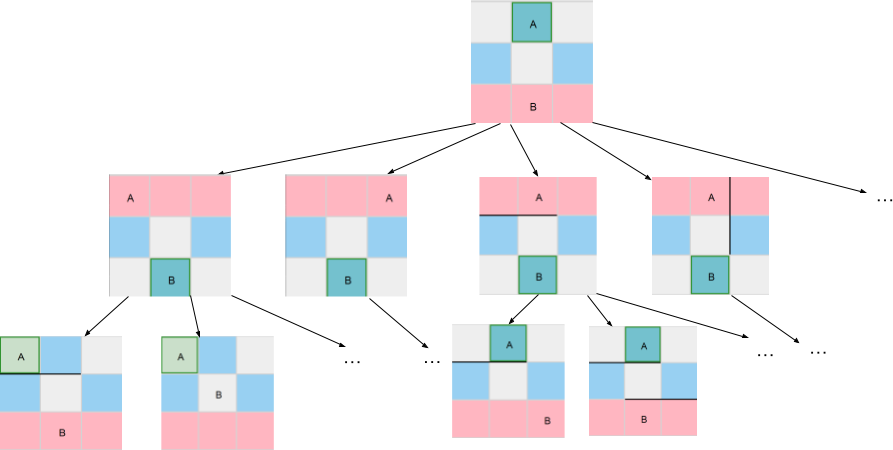
\includegraphics[scale=0.45]{../img/GameBoard/game_tree.png}
    \caption{A partial game tree for a 3x3 game board.}
    \label{fig:GameTree}
\end{figure}

As depicted in Figure \ref{fig:GameTree}, the root node of the game tree consists of player A located in the cell $C_{1, b}$ making a choice for the first move which may be one of pawn movement or wall placement. The nodes at a depth of 1 represent all possible game states as a result of moves made by player A and so on.


\subsection{Branching Factor}
\label{BranchingFactor}

The branching factor of a Game-tree is the number of child nodes of each node, or in other words, the number of possible moves a player at their turn can make, given the game state.

In Figure \ref{fig:GameTree}, player A makes the first move. A has \textbf{3} places to move their pawn to and \textbf{8} places to put one of their walls at. So, the root node has a branching factor of \textbf{11}.

The branching factor is greatly influenced by the state of the board in Quoridor, i.e the location of the pawn of the player, the location of the pawn of the opponent and the walls placed on the board.

As an example, the figure below represents a game states with the maximum and minimum branching factors:

\begin{figure}[!ht]
    \begin{subfigure}{0.4\textwidth}
      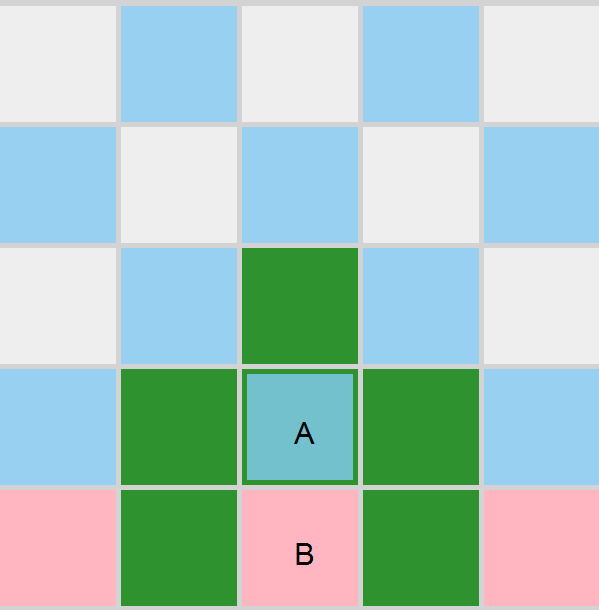
\includegraphics[width=\textwidth]{../img/GameBoard/maximum_branching_factor.png}
      \caption{Maximum : 37}
      \label{fig:MaxBranchingFactor}
    \end{subfigure}
    \hfill
    \begin{subfigure}{0.4\textwidth}
      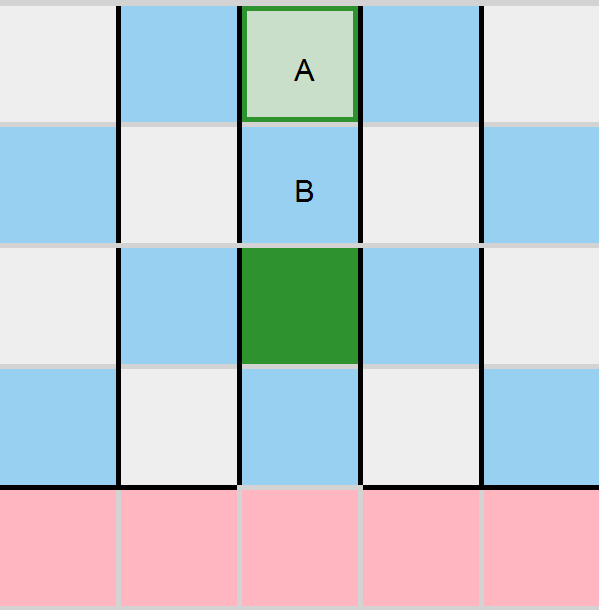
\includegraphics[width=\textwidth]{../img/GameBoard/minimum_branching_factor.png}
      \caption{Minimum : 1}
        \label{fig:MinBranchingFactor}
    \end{subfigure}
    \caption{Branching factor differences}
\end{figure}

As depicted by Figure \ref{fig:MaxBranchingFactor}, player A has 5 possible places to move their pawn to. No walls have been placed so far, so player A can also place one of their walls in any groove.

For a board of size NxN with no walls placed, $N-1$ walls can be placed in each row (since each wall occupies 2 cell lengths), and there are $N-1$ rows for correct horizontal wall placements. Hence, there are $(N-1)^2$ slots for horizontal wall placements, and since the board is NxN, the total  slots for both horizontal and vertical wall placements is given by the equation:
\begin{equation}
\label{eq:WallPlacements}
    2(N-1)^2
\end{equation}

Coming back to Figure \ref{fig:MaxBranchingFactor}, since the board has no walls placed, we now see that A has $5 + 2(5-1)^2 = 37$ possible moves they can perform, ergo, the branching factor of the game state represented by Figure \ref{fig:MaxBranchingFactor} is \textbf{37}, which is also the maximum branching factor for board sized 5x5.

However, in Figure \ref{fig:MinBranchingFactor}, player A has no available slot for wall-placement, and the already-placed walls block A from moving anywhere except for cell \textbf{$C_{3, c}$}. Hence, the branching factor for the game state represented by Figure \ref{fig:MinBranchingFactor} is \textbf{1}.

\subsubsection{Average Branching Factor}

In Sub-Section \ref{BranchingFactor}, we saw that the branching factor is not uniform due to factors like wall-placements and positioning of players greatly influencing it.

We, therefore, would like to estimate an average branching factor for boards of different dimensions to see if varying board dimension has any effect in the average branching factor.

We already know from Equation \ref{eq:WallPlacements} that the maximum branching factor of the game tree is exponential in order of $N$ and from Figure \ref{fig:MinBranchingFactor}, we can deduce that the minimum branching factor is 1 (since we can replicate a similar game state for any dimension).

To find an estimate of the average branching factor $B_{avg}$, we propose Algorithm \ref{alg:AverageBranchingFactor}, which runs N simulations between 2 agents, keeping a track of the total game states encountered and the total moves made by agents, and averaging their values.

\begin{algorithm}[!ht]
\caption{Average branching factor}
\label{alg:AverageBranchingFactor}
\DontPrintSemicolon
\SetKwInOut{Input}{input}\SetKwInOut{Output}{output}
\SetKwFunction{FMain}{AvgBranchingFactor}
\SetKwProg{Fn}{Function}{:}{}
\Fn{\FMain{agent1, agent2, simulations}}{
    \Input{Two agents and number of simulations}
    \Output{Average branching factor}
    SumOfAverages $\gets$ 0\;
    \For{i $\gets$ 1 \KwTo simulations}{
        State $\gets$ Initialize()\;
        GamePossibleMoves $\gets$ 0\;
        GameMovesMade $\gets$ 0\;
        Agents $\gets$ [agent1, agent2]\;
        AgentIndex $\gets$ 0\;
        \While{State is not Terminal}{
            Agent $\gets$ Agents[AgentIndex]\;
            AgentIndex $\gets$ (AgentIndex + 1) \% 2\;
            GamePossibleMoves $\gets$ GamePossibleMoves + Length(State.PossibleMoves())\;
            Move $\gets$ Agent.GetMove(State)\;
            State $\gets$ State.Apply(Move)\;
            GameMovesMade $\gets$ GameMovesMade + 1\;
        }
        GameAverage $\gets$ GamePossibleMoves / GameMovesMade\;
        SumOfAverages $\gets$ SumOfAverages + GameAverage\;
    }
    \KwRet SumOfAverages / simulations\;
}
\end{algorithm}

We then simulate \textbf{1000} games between \textbf{Minimax} and \textbf{Semi-random} agents, each for boards of dimensions 3, 5, 7 and 9, and for depths 1, 2 and 3, and the results of the average branching factor can be seen in Figure \ref{fig:BranchingFactor}.

\begin{figure}[!ht]
    \centering
    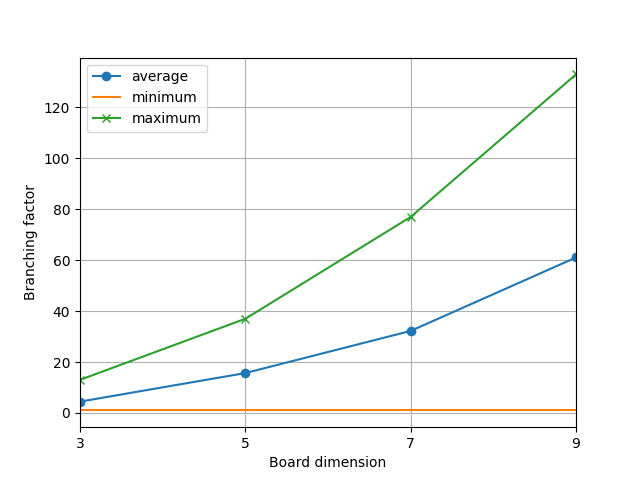
\includegraphics[scale=0.6]{../img/branching_factor.png}
    \caption{Branching factor for boards of different sizes}
    \label{fig:BranchingFactor}
\end{figure}

From Figure \ref{fig:BranchingFactor}, like with the maximum branching factor, we can see a similar exponential trend of the average branching factors in order of $N$. Furthermore, based on only the four dimensions and their averages and maximum branching factors, the average branching factor seems to be almost half the maximum branching factor.

The average branching factor for board of dimension 9x9 was about \textbf{61}, which is very close to the value proposed by \citep{Glendenning2002MasteringQ} which was 60.

\section{State space complexity}

The state space complexity is a measure of a game complexity and refers to the total number of possible states in a game. For example, for illustration with the game of Tic-Tac-Toe, there are 9 squares, each being one of X, O or empty. The state space complexity for Tic-Tac-Toe can be written as $3^9 = 19,638$. Of course, this takes into account the illegal positions as well such as all Xs or all Os and hence can be considered as an upper bound on the state space complexity. However, especially in complex games such as Chess and Quoridor with many possible states, rules and illegal positions, exact state space complexity is difficult to estimate and a way to define the complexity is through an upper bound.  

In Quoridor, this includes all the possible positions of both players' pawns on the board and all the possible configurations of walls. It is extremely difficult to find an exact value because we also need to account for wall placement rules \ref{WallRules} and pawn movement rules \ref{PlayerMoveRules}. Because of this, we loosen the regulations to come up with an upper-bound.

In \citep{Mertens2006Quoridor}, the author has determined the state space complexity for a specific board of dimension 9x9. In this thesis, we generalize the complexity evaluation to a general board of size NxN.

For a board of Dimension NxN, the first pawn can be placed in $N^2$ possible locations. After the first pawn is placed in the board, the second pawn now has $N^2-1$ possible locations to be placed into. So, the total number of ways for pawn placement, $S_p$ is given by
\begin{equation}
    S_p = N^2(N^2 - 1)
\end{equation}

As for walls, from Equation \ref{eq:WallPlacements}, we know that there are $2(N-1)^2$ ways of placing walls on the board, both horizontally and vertically. Since we know that each wall occupies 2 cells, we will use assumption made by the author of \citep{Mertens2006Quoridor} that placing the wall anywhere in the board takes away the possibility of placing walls at 4 different places. As each placed wall takes two cells, placing a wall, for e.g., horizontally, means that further walls cannot be placed in the location of the wall, walls starting from the cell left and right to the cell of the wall and a wall placed vertically through the placed wall. Every placed wall hence takes away 4 spaces for wall placement. The same example is also valid for a vertically placed wall. Hence assuming that $j$ walls are placed from a given game state, the total number of branches of the game state for wall placement may be $2(N-1)^2 - 4j$,

Furthermore, for a given board dimension (e.g., NxN), there is a fixed number of walls in the game $N_w$. For example, for the standard 9x9 board with 81 total squares, $N_W = 20$. We can extrapolate the number of walls that may be available for boards of other dimensions too based on the number of squares. For example, for 3x3 board, $N_W = 2$, for 5x5 board $N_w = 8$, for 7x7 board $N_W = 12$.

In the game tree, there may be a path where a total of $N_W$ walls are used. In such scenario, the total number of branches $L_{N_w}$ in the tree can be defined by the following equation:
\begin{equation}
    L_{N_w} = \prod_{j=0}^{N_w} (2(N-1)^2 - 4j),
\end{equation}
where, each component in the product defines the total number of states in the subsequent turn following a wall placement.

However, in the game, all the walls may not be necessarily placed. Hence, in such case, the total number of walls used may be variable and hence the total possibilities for wall placement $S_w$ is defined by the following equation:
\begin{equation}
    S_w = \sum_{i=0}^{N_w}\prod_{j=0}^{i}(2(N-1)^2 - 4j).
\end{equation}

And thus, since the game tree consists of the possibilities of both pawn movement and wall placement, the total state space complexity is given by $S = S_w * S_p$. \citep{Mertens2006Quoridor}

\begin{equation}
    S = N^2(N^2 -1) \times \sum_{i=0}^{N_w}\prod_{j=0}^{i}(2(N-1)^2 - 4j).
\end{equation}

\begin{figure}[!ht]
    \centering
    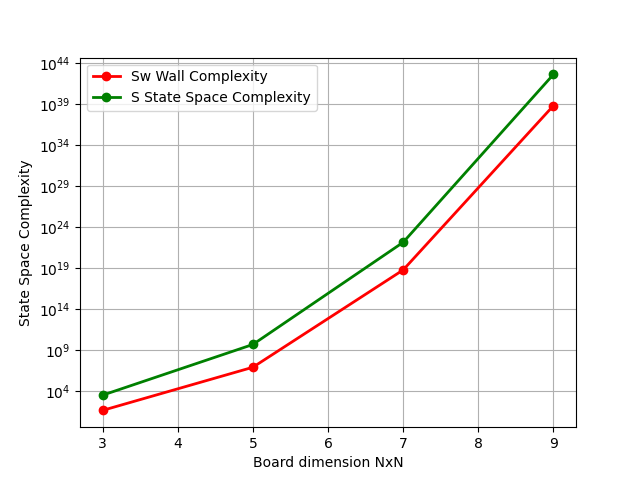
\includegraphics[width=.9\linewidth]{../img/Complexity.png}
    \caption{Complexity vs Board Dimension}
    \label{fig:complexity}
\end{figure}

In Figure \ref{fig:complexity}, we can see the log plot of the state space complexity of wall placement and the game when varied with the dimension of the game (i.e., 3x3, 5x5, 7x7 and 9x9). In the figure, we can see the state space of the game grows exponentially with the increase in the board dimension. Moreover, the state space complexity is dominated by the complexity of the wall placement as seen by the difference between the two curves.


\section{Game tree complexity}

The game-tree complexity of a game, as defined in \citep{Allis1994Searching}, is another measure of a game complexity alongside the state-space complexity. The authors define a game tree complexity as "\textit{the number of leaf nodes in the solution search tree of the initial position(s) of the game}".

The game tree complexity refers to the number of possible games that can be played. Unlike the state space complexity, which measures the total number of possible states of the game from the starting position, the game tree complexity measures the size of the game tree. The size of the game tree or the game-tree complexity typically is larger than the state space complexity because a game state (counted only once in the state space complexity) can arise through multiple games (counted multiple times in the game tree complexity).

An example of the game tree complexity can be illustrated through the game of tic-tac-toe. In the game tree, player A has 9 positions to put the mark (e.g., X or 0) on. Subsequently, in the second move, player B can put the mark on 8 spaces as one has been taken away in the first move and so on. Hence, the game tree complexity of tic-tac-toe can be defined as $9 \times 8 \times \cdots \times 1 = 9! = 362380$. In comparison to the state space complexity of tic-tac-toe, the game tree complexity is higher as a position arising through different orders of play is counted as one state with the state space complexity and multiple game tree positions with the game tree complexity. 


In complex games like Quoridor, the game-tree complexity $G$ can be estimated by raising the average branching factor $B_{avg}$ to a power of the total number of moves by the players $D_{avg}$ \citep{Mertens2006Quoridor}, which is given by the following equation: 
\begin{equation}
    G = B_{avg}^{D_{avg}}
\end{equation}

The average depth $D_{avg}$ simulated for different dimensions of the game can be found below:
\begin{align*}
    &D_{avg, \text{3x3}} = 11\\
    &D_{avg, \text{5x5}} = 47\\
    &D_{avg, \text{7x7}} = 72\\
    &D_{avg, \text{9x9}} = 97
\end{align*}

Subsequently, we can now determine the game tree complexity based on the determined $B_{avg}$ and $D_{avg}$. The game tree complexity for different dimensions can be written as:
\begin{align*}
    &G_\text{3x3} = 8.58 * 10^9\\
    &G_\text{5x5} = 9.94 * 10^{58}\\
    &G_\text{7x7} = 5.56 * 10^{113}\\
    &G_\text{9x9} = 1.50 * 10^{173}
\end{align*}

From this, we can infer that the game state complexity for Quoridor, like the state space complexity, also increases exponentially with the increase in the dimension of the game.


\section{Comparison with other games}

\begin{table}[ht]
    \centering
     \begin{tabular}{|c|c|c|c|}\hline
          & $\log_{10}(S)$ & $\log_{10}(G)$ & $B_{avg}$\\ \hline 
          Tic-tac-toe  & 3   & 5   & 4    \\ \hline
  \textbf{Quoridor 3x3} & 3  & 10  & 8  \\ \hline
          Connect-four & 13  & 21  & 4    \\ \hline
  \textbf{Quoridor 5x5} & 10  & 59 & 18  \\ \hline
  \textbf{Quoridor 7x7}  & 22  & 113 & 38  \\ \hline
          Chess        & 44  & 123 & 35   \\ \hline
  \textbf{Quoridor 9x9}     & 42  & 173 & 61  \\ \hline        
          Go           & 170 & 360 & 250 \\ \hline
     \end{tabular}
     \caption{State space, game tree and branching factor comparison between well-known games}
     \label{tab:comparison}
 \end{table}

 In the Table \ref{tab:comparison}, we present the logarithm of the state space complexity ($\log(S)$), the game state complexity ($\log(G)$) and the average branching factor ($B_avg$) of some popular games from the literature \citep{Mertens2006Quoridor}.

 As we can see from the above table, Quoridor with board dimension 3x3 has the state space complexity and the game tree complexity similar to that of Tic-tac-toe. It can also be inferred that the Quoridor game with dimension 9x9 has similar complexity compared to chess.
 